% 2009 年浙江卷文科第 19 题：DC⊥平面 ABC，EB∥DC，AC=BC=EB=2DC=2，
% ∠ACB=120°，P、Q 分别为 AE、AB 的中点。
% 来源 PDF：普通高考/2009/2009浙江文.pdf，SHA-256 8e609d19459cb4234a4d6dd9db5be5c8cc9af2169c00d4337b3988089cfb0709。
% 原页：第 2 页第 1 栏上部，书页码 568。
% 重绘依据：按斜二测投影重绘；D 在 C 正上方、E 在 B 正上方，DC 与 EB 均画成
%   竖直；C 在底面 ABC 内，故 CA、CB、CD 为虚线，其余可见棱为实线。
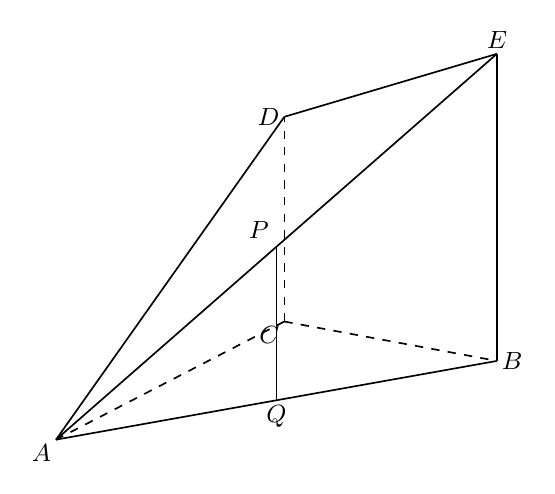
\begin{tikzpicture}[semithick, every node/.style={inner sep=1.5pt, font=\small}]
  \coordinate (A) at (0,0);
  \coordinate (B) at (5.6,1.0);
  \coordinate (C) at (2.9,1.5);
  \coordinate (D) at (2.9,4.1);
  \coordinate (E) at (5.6,4.9);
  \coordinate (P) at (2.8,2.45);
  \coordinate (Q) at (2.8,0.5);

  % 可见棱
  \draw (A) -- (B);
  \draw (A) -- (D);
  \draw (A) -- (E);
  \draw (D) -- (E);
  \draw (E) -- (B);
  \draw (P) -- (Q);

  % 被遮挡的棱
  \draw[dashed] (C) -- (A);
  \draw[dashed] (C) -- (B);
  \draw[dashed] (C) -- (D);

  % 标签
  \node[below left] at (A) {$A$};
  \node[right] at (B) {$B$};
  \node[below left] at (C) {$C$};
  \node[left] at (D) {$D$};
  \node[above] at (E) {$E$};
  \node[above left=1pt] at (P) {$P$};
  \node[below] at (Q) {$Q$};
\end{tikzpicture}
